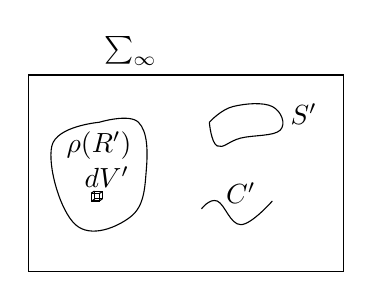
\begin{tikzpicture}

\draw  (-1.5,1.5) rectangle (2.5,-1);
\draw  plot[smooth, tension=.7] coordinates {(-0.6,0.9) (-1.2,0.6) (-0.9,-0.4) (-0.2,-0.3) (0,0.3) (-0.1,0.9) (-0.6,0.9)};
\node at (-0.6,0.6) {$\rho(R')$};
\draw  (-0.7,0) node (v2) {} rectangle (-0.6,-0.1) node (v4) {};
\draw  (-0.6589,0.0266) node (v1) {} rectangle (-0.5589,-0.0734) node (v3) {};
\draw (-0.5547,0.0204) -- (-0.5962,-0.0034);
\draw (-0.6556,-0.0746) -- (-0.6912,-0.0984);
\draw (v1.center) -- (v2.center);
\draw (v3.center) -- (v4.center);
\node at (-0.5,0.2) {$dV'$};
\node at (-0.2,1.8) {$\sum_\infty$};
\draw  plot[smooth, tension=.7] coordinates {(0.8,0.9) (1.1,1.1) (1.6,1.1) (1.7,0.8) (1.2,0.7) (0.9,0.6) (0.8,0.9)};
\draw  plot[smooth, tension=.7] coordinates {(0.7,-0.2) (0.9,-0.1) (1.2,-0.4) (1.6,-0.1)};
\node at (2,1) {$S'$};
\node at (1.2,0) {$C'$};
\end{tikzpicture}